\documentclass[12pt]{article}
\usepackage{amsmath,amssymb,amsthm}
\usepackage{graphicx,mathabx}
\usepackage{xcolor}
\usepackage{tikz}
\usepackage{placeins}
\usepackage{lipsum}
\usepackage[shortlabels]{enumitem}
\usepackage{placeins}
\usepackage[makeroom]{cancel}
\newcommand\tab[1][1cm]{\hspace*{#1}}
\def\blankpage{%
      \clearpage%
      \thispagestyle{empty}%
      \addtocounter{page}{-1}%
      \null%
      \clearpage}
\begin{document}
\title{TCSS 343 - Week 5}
\author{Jake McKenzie}
\maketitle
\noindent\centerline{\textbf{Greedy Algorithms}}\\\\\\\\\\\\\\\\
\begin{center}
    ``We don't much care if you don't approve of the software we write." \\$\dots$\\ Eric Hughes
\end{center}
\begin{center}
    ``Greedy algorithms: do the thing that looks best right now, and repeat until nothing looks good anymore or you're forced to stop." \\$\dots$\\ Jeremy Kun
\end{center}
\begin{center}
    ``The best programs are the ones written when the programmer is supposed to be working on something else." \\$\dots$\\ Melinda Varian
\end{center}
\newpage

\includegraphics[width=\textwidth]{svenborgia.jpg}\\
\noindent You want to invite as many people to your party as possible. 
But, there’s a catch: you don’t quite trust the
other diplomats, all of whom speak multiple languages. 
So, you’d like to make sure that you can understand
what everyone is saying at your party. As the Canadian 
ambassador to Svenborgia, you speak English,
French, and Svenborgian. You want to make sure 
that no two of your party guests speak the same language,
other than the three you speak. For each diplomat, 
you have a list of of every “foreign” language (i.e.,
other than English, French, or Svenborgian) that they 
speak. We refer to this as the International Party
Guest, or IPG, problem.\\\\
For example: suppose there 
are three diplomats. If 
diplomat 1 speaks language 
1, diplomat 2 speaks
languages 2 and 3, and diplomat 
3 speaks languages 1, 3, and 4, we 
would represent this instance as
\{\{1\}, \{2, 3\}, \{1, 3, 4\}\}. 
The optimal solution to this instance 
is to invite diplomat 1 and diplomat 2.\\\\
Consider the two following greedy algorithms 
designed to maximize the number of guests you 
can invite. For each, determine whether the 
algorithm is optimal. If it is, briefly sketch a 
proof of optimality. If
it’s not, give a counterexample(next page).
\newpage
\noindent 0. \textbf{Greedy Strategy 0:} if no two diplomats 
speak the same foreign language, invite them all. 
Otherwise, invite the diplomat who speaks the fewest 
languages only if they don't share a language with
the next diplomat in the invite pool, and recurse.\\\\\\\\\\\\
1. \textbf{Greedy Strategy 1:} if no two diplomats 
speak the same foreign language, invite them all. 
Otherwise, remove the diplomat who speaks 
more than half the possible languages, and recurse.\\\\\\\\\\\\
2. \textbf{Greedy Strategy 2:} if no two diplomats 
speak the same foreign language, invite them all. Otherwise,
remove the diplomat who speaks the most languages, and recurse.\\\\\\\\\\\\
3. \textbf{Greedy Strategy 3:} if no two diplomats speak the 
same foreign language, invite them all. Otherwise,
invite the diplomat who speaks the fewest languages, 
remove all other diplomats who share a language
with the one you just invited, and recurse.
\newpage
\centerline{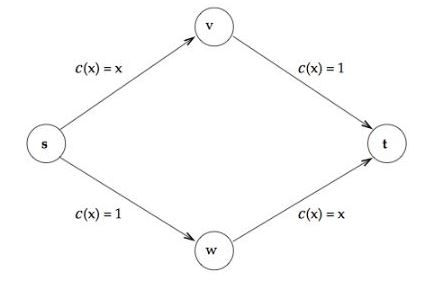
\includegraphics[scale = .7]{braess1.jpg}}
\noindent 4. We have a group of people commuting home from a vertex $s$ to $t$.
Let the edges with cost $c(x) = x$ be the proportion
of drivers traveling along those edges at any given time. 
Let's say drivers employ a greedy strategy.
Find the total cost (units are hours) to get home for the drivers along this graph.\\\\\\\\
\centerline{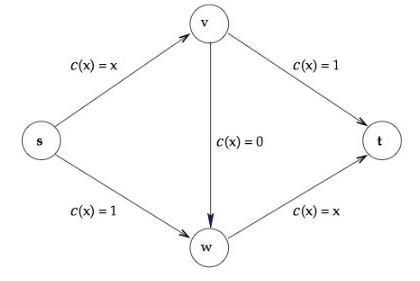
\includegraphics[scale = .7]{braess2.jpg}}
5. Let's say the same group of people were traveling along the same path,
but all of a sudden Google invents a teleportation device between vertex $v$ to $w$ which
adds no additional time to their commute,
what now is the total time it takes to get home for the drivers along this graph?\\\\\\\\
6. Why must we be careful when implementing greedy algorithms? When do greedy algorithms fail?
\newpage
\centerline{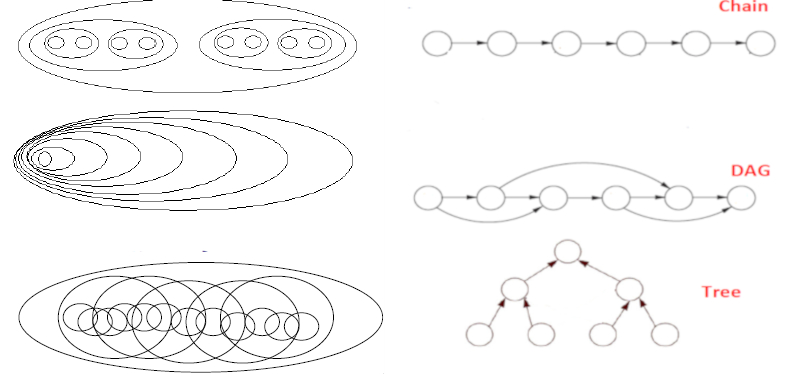
\includegraphics[scale = 2]{prob3.jpg}}
\noindent 7. Above are venn diagrams and graphs that match to the three algorithmic design techniques covered in class so far. 
Please match each design technique to their venn diagram and graph.
\begin{enumerate}[a)]
    \item \textbf{Dynamic Programming:} Overlapping sub-problems, recursion is forbidden, many choices for subproblems
    \item \textbf{Greedy:} A sub-problem defiines the next one with a single (greedy) binary choice.
    \item \textbf{Divide and Conquer:} Non-overlapping subproblems, recursion can and is often used.
\end{enumerate}
\newpage
\centerline{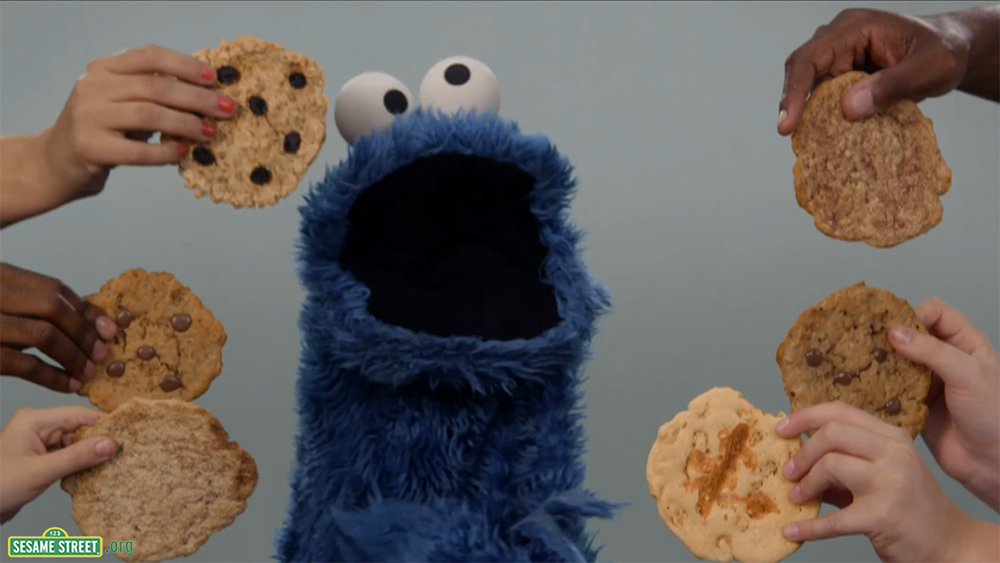
\includegraphics[width=\textwidth]{cookies.jpg}}
\noindent 8. You are given a sequence of $C$ cookies rated by their tastiness factor. Partition the sequence into segments such that the sum of the tastiness in each gobble full is smaller than a given cap $H$ (handfull factor). Give an algorithm that minimizes the number of segments. (This was a question asked by Facebook on Glassdoor. They wanted it done in better than $n \log{n}$ but let's stick to a greedy approach)
\newpage \noindent 9. Assume the tastiness factor for the cookies $C$ could be negative, meaning they're fake cookies that are actually frutis and vegetables disguised as cookies. Come up with a sequence of cookies $C$ with a handfull factor $H$ where your greedy algorithm does not come up with the optimal solution.\\\\\\\\\\\\\\\\\\\\\\\\
A. Consider the cashier problem you saw in class, our coin values are:
$\{1,$ $2,$ $4,$ $8,$ $16,$ $\dots$ $,2k\}$, for some positive integer $k$. Give a modified cashier's algorithm that runs in $O(\log{n})$
to solve the problem if the value to be paid is $y < 2^{k+1}$.
\newpage
\noindent B. Construct a greedy algorith that finds the postive integer solution $(x$, $y$, $z$, $a$, $b)$ for which\\\\
$$\frac{1}{x}+\frac{1}{y}+\frac{1}{z}+\frac{1}{a}+\frac{1}{b}=1$$
Avoid the trivial solution where $x=y=z=a=b=5$ such that $x\neq y \neq z \neq a \neq b$.\\
(\textbf{Remark:} There are 72 tuples that satisfy this equation.)
\newpage
\noindent C. Find which coin you could remove from the U.S. coinage system as to keep the greedy cashier algorithm
from returning the optimal result. To show this you need to find the coin and counter example for each.\\\\\\\\\\\\\\\\\\\\\\\\
D. Which coins could we add which would make the coin system in the U.S. MORE canonical, which means simply, it returns even fewer coins as change? (HINT because this is harder:
The numbers are prime and less than 11.)
\newpage
\noindent E. Consider the Gerrymandering problem: Suppose we have a set of $n$ precincts $P_1$, $P_2$, $\dots$ , $P_n$,
each containing $m$ registered voters. We’re supposed to divide these precincts into two districts,
each consisting of $\frac{n}{2}$ of the precincts. Now, for each precinct, we have information
on how many voters are registered to each of two political parties. We’ll say that the set of
precincts is susceptible to gerrymandering if it is possible to perform the division into two
districts in such a way that the same party holds a majority in both districts
\\\\
Give an algorithm to determine whether a given set of precincts is susceptible to gerrymandering;
the running time of your algorithm should be polynomial in $n$ and $m$
\\\\
Example: Suppose we have $n$ $=$ $4$ precincts, and the following information on registered
voters: Precinct 1 has 55 voters for party A, $45$ voters for party B; Precinct 2 has $43$ for A,
$57$ for B; Precinct 3 has $60$ for A, $40$ for B; Precinct 4 has $47$ for A, $53$ for B.
\\\\
This set of precincts is susceptible since, if we grouped precincts $1$ and $4$ into one district,
and precincts 2 and 3 into the other, then party A would have a majority in both districts.
\blankpage
\newpage
\noindent F. Let $G$ $=$ $(V,E)$ be an undirected graph. A vertex cover for $G$ is a subset
$S$ $\subseteq$ $V$ such that every edge in $E$ is incident to at least one vertex in $S$.
Consider the following algorithm for finding a vertex cover for $G$. First,
order the vertices in $V$ by decreasing order of degree. Next execute the following
step until all edges are covered. Pick a vertex of highest degree that
is incident to at least one edge in the remaining graph, add it to the cover,
and delete all edges incident to that vertex. Show that this greedy approach
does not always result in a vertex cover of minimum size.
\end{document}